\subsection{Clinical-development landscape: curation-corrected trial mining of the gated surfaceome}
\label{sec:clintrials}
Expression gating ranks antigens by tumour selectivity, but a practical question
remains: how much clinical development already targets the gated surfaceome, and
how crowded are the seven AND-gate antigens? We audited all @NGENES@ gene-set
genes against ClinicalTrials.gov (API v2) in three tiers: \textbf{strict}
(gene-symbol token in intervention names, restricted to oncology conditions),
\textbf{broad} (full-text symbol mention with a modality keyword), and a curated
\textbf{alias} tier for the seven AND-gate antigens and four clinical references
(e.g.\ HER2 for ERBB2, BCMA for TNFRSF17, claudin-18.2/zolbetuximab for CLDN18),
capturing trials whose agents do not carry the raw gene symbol.

\paragraph{Calibration.} The tier was gated before any claim: CD19 must be
highly visible (observed @CD19VER@ verified trials), and the intracellular
noise controls POLR2A and RPS3 must be silent (observed @NEGSUM@). Both gates
passed. Two further controls are instructive: PCNA attracted @PCNAVER@ genuine
targeted trials (the AOH1996 PCNA-inhibitor program), and PSMA1's three hits
were all PSMA (FOLH1) radioligand trials, a pure name collision.

\paragraph{Acronym noise is half the raw signal.} The raw oncology-restricted
strict tier suggested that gated antigens carry more development than background
(Mann--Whitney $p = @RAWMWP@$). We then title-inspected every one of the
@NINSPECT@ genes with at least one hit: @NCOLL@ were acronym collisions or
biomarker-only studies -- NMB matched \emph{neuromuscular blockade} anesthesia
trials, MAL matched \emph{methyl aminolevulinate} photodynamic therapy, LAT
matched \emph{local ablative treatment}, GP2 matched a HER2-derived peptide
vaccine (the GP2 peptide), AFM matched the CD30$\times$CD16A bispecific AFM13,
and S100A9 matched calprotectin diagnostics. After curation the enrichment
collapses to a non-significant trend (@NGEN@ genuine genes; curated MW
$p = @VERMWP@$; any verified development in @GANY@ gated vs @BANY@ background,
Fisher $p = @VFISHP@$; recruiting-status subset $p = @VACTMWP@$). Trial-landscape
mining by gene symbol is therefore uninterpretable without per-gene curation,
and we report curated counts throughout.

\paragraph{What development the gated set does carry.} The verified gated
development concentrates in already clinically validated targets -- EGFR (148),
MSLN (41), HLA-A (25 HLA-A-restricted vaccines/TCRs), TACSTD2 (16, the
sacituzumab era), EPCAM (10), CA9 and CEACAM5 (7 each) -- while background's
verified development is KRAS (34), ALK (16), and three small programs. Gating
thus recovers the field's validated surface targets at 2.4$\times$ the
background gene rate, a consistency check rather than a novelty claim.

\paragraph{The AND-gate antigens.} The alias tier (Table~\ref{tab:clintrials})
shows a split landscape. MSLN is clinically mature (@MSLNALIAS@ alias trials,
@MSLNACT@ active or recruiting; @MSLNSTRICT@ strict). CLDN18 carries
@CLDN18ALIAS@ alias-tier trials of the zolbetuximab generation yet \emph{zero}
strict-tier agents -- no intervention name carries the CLDN18 symbol, the same
alias-invisibility as TNFRSF17 (@BCMAALIAS@ alias, 0 strict; agents are
BCMA-named). CLDN6, PSCA, and CA9 carry modest pipelines (@CLDN6ALIAS@,
@PSCAALIAS@, @CA9ALIAS@ alias trials), while CA12 and SLC39A6 are near-empty
(@CA12ALIAS@ and @SLCALIAS@). All seven remain far below the reference ceiling
(CD19 $\geq$@CD19ALIAS@, ERBB2/HER2 $\geq$@ERBB2ALIAS@, FOLR1 @FOLR1ALIAS@).
Combined with the free-loss escape audit (Sec.~\ref{sec:constraint}), CA12,
CLDN6, and SLC39A6 occupy a rare quadrant: low escape cost for the tumour
\emph{and} near-zero development crowding. In total @NUNIQNCT@ unique
NCT-number-backed trial records were individually fetched and used here.

\begin{table}[t]
\centering\small
\caption{ClinicalTrials.gov landscape for the seven AND-gate antigens and four
clinical references. Alias tier uses curated aliases; active = recruiting /
active-not-recruiting / enrolling / not-yet-recruiting; verified strict =
symbol-token intervention-name hits surviving acronym-collision curation;
$\geq$ marks queries truncated at the 1000-record page cap.}
\label{tab:clintrials}
\begin{tabular}{llrrr}
\hline
Gene & Class & Alias trials & Active & Verified strict \\
\hline
@ALIASROWS@
\hline
\end{tabular}
\end{table}

\begin{figure}[t]
\centering
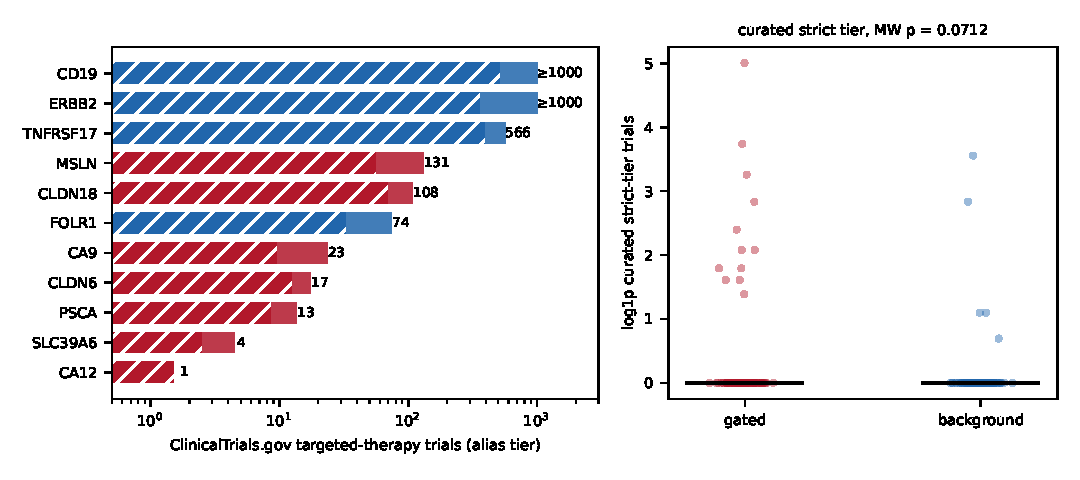
\includegraphics[width=\textwidth]{clintrials_fig.pdf}
\caption{\textbf{a} Alias-tier trial counts for the AND-gate antigens (red) and
clinical references (blue); hatched segments are active/recruiting; $\geq$ marks
capped queries. \textbf{b} Curated strict-tier counts across the 99-gene gated
surfaceome vs the 98-gene background (median bars; Mann--Whitney
$p = @VERMWP@$): after acronym-collision curation the gated set shows only a
non-significant excess of verified target-directed development.}
\label{fig:clintrials}
\end{figure}
